\documentclass[conference]{IEEEtran}
\IEEEoverridecommandlockouts
\usepackage{cite}
\usepackage{balance}
\usepackage{amsmath,amssymb,amsfonts}
\usepackage{graphicx}
\usepackage{textcomp}
\usepackage{xcolor}
\usepackage{booktabs}
\usepackage{algorithm}
\usepackage{algorithmic}
\usepackage{tikz}
\usetikzlibrary{positioning,arrows.meta,fit,calc}
\usepackage[hidelinks]{hyperref}
\newcommand{\NInst}{30}
\newcommand{\NFeasInst}{30}
\newcommand{\NBinding}{12}
\newcommand{\MeanFeasAssign}{45.0}
\newcommand{\Shots}{32}
\newcommand{\UniBits}{0.00033}
\newcommand{\UniOneHot}{0.0169}
\newcommand{\ExactMs}{0.90}
\newcommand{\SAOpt}{10.0}
\newcommand{\SAFeas}{83.3}
\newcommand{\SAMs}{2.3}
\newcommand{\GreedyOpt}{93.3}
\newcommand{\GreedyFeas}{100.0}
\newcommand{\QuboExact}{93.3}
\newcommand{\QXMeanOnePopt}{0.004}
\newcommand{\QXMeanOnePfeas}{0.074}
\newcommand{\QXMeanOneSucc}{12.2}
\newcommand{\QXMeanOneArgmax}{36.7}
\newcommand{\QXMeanOneNfev}{96}
\newcommand{\QXMeanOneMs}{0.29}
\newcommand{\QXMeanTwoPopt}{0.011}
\newcommand{\QXMeanTwoPfeas}{0.249}
\newcommand{\QXMeanTwoSucc}{27.6}
\newcommand{\QXMeanTwoArgmax}{40.0}
\newcommand{\QXMeanTwoNfev}{479}
\newcommand{\QXMeanTwoMs}{4.22}
\newcommand{\QXMeanThreePopt}{0.024}
\newcommand{\QXMeanThreePfeas}{0.439}
\newcommand{\QXMeanThreeSucc}{48.2}
\newcommand{\QXMeanThreeArgmax}{26.7}
\newcommand{\QXMeanThreeNfev}{721}
\newcommand{\QXMeanThreeMs}{4.03}
\newcommand{\QXMeanFourPopt}{0.040}
\newcommand{\QXMeanFourPfeas}{0.547}
\newcommand{\QXMeanFourSucc}{63.7}
\newcommand{\QXMeanFourArgmax}{40.0}
\newcommand{\QXMeanFourNfev}{750}
\newcommand{\QXMeanFourMs}{8.71}
\newcommand{\QXYMeanOnePopt}{0.054}
\newcommand{\QXYMeanOnePfeas}{0.734}
\newcommand{\QXYMeanOneSucc}{67.1}
\newcommand{\QXYMeanOneArgmax}{3.3}
\newcommand{\QXYMeanOneNfev}{272}
\newcommand{\QXYMeanOneMs}{0.83}
\newcommand{\QXYMeanTwoPopt}{0.093}
\newcommand{\QXYMeanTwoPfeas}{0.722}
\newcommand{\QXYMeanTwoSucc}{77.8}
\newcommand{\QXYMeanTwoArgmax}{13.3}
\newcommand{\QXYMeanTwoNfev}{741}
\newcommand{\QXYMeanTwoMs}{2.97}
\newcommand{\QXYMeanThreePopt}{0.143}
\newcommand{\QXYMeanThreePfeas}{0.743}
\newcommand{\QXYMeanThreeSucc}{81.9}
\newcommand{\QXYMeanThreeArgmax}{16.7}
\newcommand{\QXYMeanThreeNfev}{750}
\newcommand{\QXYMeanThreeMs}{3.73}
\newcommand{\QXYMeanFourPopt}{0.215}
\newcommand{\QXYMeanFourPfeas}{0.795}
\newcommand{\QXYMeanFourSucc}{88.4}
\newcommand{\QXYMeanFourArgmax}{40.0}
\newcommand{\QXYMeanFourNfev}{750}
\newcommand{\QXYMeanFourMs}{5.53}
\newcommand{\QXCvarOnePopt}{0.005}
\newcommand{\QXCvarOnePfeas}{0.132}
\newcommand{\QXCvarOneSucc}{14.6}
\newcommand{\QXCvarOneArgmax}{23.3}
\newcommand{\QXCvarOneNfev}{108}
\newcommand{\QXCvarOneMs}{0.37}
\newcommand{\QXCvarTwoPopt}{0.019}
\newcommand{\QXCvarTwoPfeas}{0.294}
\newcommand{\QXCvarTwoSucc}{44.0}
\newcommand{\QXCvarTwoArgmax}{63.3}
\newcommand{\QXCvarTwoNfev}{577}
\newcommand{\QXCvarTwoMs}{54.22}
\newcommand{\QXCvarThreePopt}{0.037}
\newcommand{\QXCvarThreePfeas}{0.356}
\newcommand{\QXCvarThreeSucc}{65.7}
\newcommand{\QXCvarThreeArgmax}{70.0}
\newcommand{\QXCvarThreeNfev}{728}
\newcommand{\QXCvarThreeMs}{793.23}
\newcommand{\QXCvarFourPopt}{0.060}
\newcommand{\QXCvarFourPfeas}{0.376}
\newcommand{\QXCvarFourSucc}{78.4}
\newcommand{\QXCvarFourArgmax}{66.7}
\newcommand{\QXCvarFourNfev}{706}
\newcommand{\QXCvarFourMs}{5.47}
\newcommand{\QXYCvarOnePopt}{0.067}
\newcommand{\QXYCvarOnePfeas}{0.720}
\newcommand{\QXYCvarOneSucc}{82.7}
\newcommand{\QXYCvarOneArgmax}{6.7}
\newcommand{\QXYCvarOneNfev}{241}
\newcommand{\QXYCvarOneMs}{0.83}
\newcommand{\QXYCvarTwoPopt}{0.099}
\newcommand{\QXYCvarTwoPfeas}{0.712}
\newcommand{\QXYCvarTwoSucc}{93.9}
\newcommand{\QXYCvarTwoArgmax}{20.0}
\newcommand{\QXYCvarTwoNfev}{413}
\newcommand{\QXYCvarTwoMs}{1.78}
\newcommand{\QXYCvarThreePopt}{0.127}
\newcommand{\QXYCvarThreePfeas}{0.672}
\newcommand{\QXYCvarThreeSucc}{97.3}
\newcommand{\QXYCvarThreeArgmax}{36.7}
\newcommand{\QXYCvarThreeNfev}{343}
\newcommand{\QXYCvarThreeMs}{1.88}
\newcommand{\QXYCvarFourPopt}{0.149}
\newcommand{\QXYCvarFourPfeas}{0.664}
\newcommand{\QXYCvarFourSucc}{98.1}
\newcommand{\QXYCvarFourArgmax}{50.0}
\newcommand{\QXYCvarFourNfev}{284}
\newcommand{\QXYCvarFourMs}{1.75}
\newcommand{\XYPfeasMin}{0.722}
\newcommand{\XYPfeasMax}{0.795}
\newcommand{\GainXYoverUni}{12.7}
\newcommand{\GainXYoverX}{5.3}
\newcommand{\ZZX}{14.0}
\newcommand{\ZZXY}{2.0}
\newcommand{\OvPairs}{2.0}
\newcommand{\ScaleMaxQ}{18}
\newcommand{\ScaleXYsix}{0.006}
\newcommand{\ScaleUnisix}{0.0017}
\newcommand{\ScaleXYmsSix}{99.4}
\newcommand{\ScaleExactSix}{8.14}
\newcommand{\ScaleQuboMin}{90}
\newcommand{\NNonBinding}{18}
\newcommand{\XYBind}{0.111}
\newcommand{\XYNonBind}{0.284}
\newcommand{\XYMin}{0.002}
\newcommand{\XYCvarMin}{0.074}
\newcommand{\XYMax}{0.796}
\newcommand{\XYCvarMax}{0.439}
\newcommand{\XBind}{0.039}
\newcommand{\XNonBind}{0.041}
\newcommand{\ScaleXYtwo}{0.694}
\newcommand{\ScaleXtwo}{0.124}
\newcommand{\ScaleXsix}{0.0009}
\newcommand{\ScaleInfeasSix}{1}
\newcommand{\ScaleXYfeasSix}{0.271}
\newcommand{\ScaleXfeasSix}{0.051}
\newcommand{\TrajInst}{10}
\newcommand{\TrajRuns}{200}
\newcommand{\TrajIdealXY}{0.172}
\newcommand{\TrajIdealX}{0.046}
\newcommand{\TrajXYOne}{0.105}
\newcommand{\TrajXOne}{0.033}
\newcommand{\TrajGlobXYOne}{0.086}
\newcommand{\TrajXYTwo}{0.058}
\newcommand{\TrajRatioOne}{3.2}
\newcommand{\NtwoLayer}{14.0}
\newcommand{\CnotLayer}{28}
\newcommand{\CnotFour}{112}
\newcommand{\ExOpt}{ABCB}
\newcommand{\ExOptCost}{80.86}
\newcommand{\ExSecond}{ABBB}
\newcommand{\ExSecondCost}{80.88}
\newcommand{\ExGap}{0.02}
\newcommand{\ExXYOpt}{0.319}
\newcommand{\ExXYSecond}{0.303}
\newcommand{\ExXYFeas}{0.982}
\newcommand{\ExXOpt}{0.049}
\newcommand{\ExXFeas}{0.681}
\newcommand{\ExNFeas}{29}
\newcommand{\NoiseXYOnePct}{0.104}
\newcommand{\NoiseXYOnePctDepth}{4}
\newcommand{\NoiseXOnePct}{0.023}
\newcommand{\NoiseXYTwoPct}{0.050}
\newcommand{\NoiseXYTwoPctDepth}{4}
\newcommand{\NoiseCvarTwoPctDepth}{2}
\newcommand{\NSeeds}{5}
\newcommand{\NPaired}{30}
\newcommand{\SeedXYMean}{0.188}
\newcommand{\SeedXYSd}{0.020}
\newcommand{\SeedXYMin}{0.168}
\newcommand{\SeedXYMax}{0.215}
\newcommand{\SeedXMin}{0.035}
\newcommand{\SeedXMax}{0.048}
\newcommand{\GMMeanFour}{0.139}
\newcommand{\GMCvarFour}{0.117}
\newcommand{\GMFeasFour}{0.815}
\newcommand{\StXYvXMaxP}{8.0\times10^{-6}}
\newcommand{\StXYvXMinP}{2.2\times10^{-8}}
\newcommand{\StXYvXWinsMin}{25}
\newcommand{\StXYvXWinsMax}{29}
\newcommand{\StXYvGMMaxP}{0.74}
\newcommand{\StXYvGMMinP}{0.19}
\newcommand{\StXYvGMWinsMin}{15}
\newcommand{\StXYvGMWinsMax}{20}
\newcommand{\PenBestLam}{0.25}
\newcommand{\PenBestPopt}{0.104}
\newcommand{\PenBestFeas}{0.401}
\newcommand{\PenGain}{2.6}
\newcommand{\SATunedOpt}{80.0}
\newcommand{\SATunedFeas}{90.0}
\newcommand{\SATunedMs}{128}
\newcommand{\ZeroPenInfeasAll}{30}
\newcommand{\LooDonorFour}{0.292}
\newcommand{\LooTrainedFour}{0.215}
\newcommand{\LooMedianFour}{0.001}
\newcommand{\LooNDonors}{2}
\newcommand{\BestFiveFour}{0.297}
\newcommand{\BestFiveEvals}{12,552}
\newcommand{\HoN}{30}
\newcommand{\HoFt}{30}
\newcommand{\HoTrainedFour}{0.163}
\newcommand{\HoFixedFour}{0.306}
\newcommand{\HoFtFour}{0.356}
\newcommand{\HoCumFour}{2,496}
\newcommand{\HoWinsFour}{24}
\newcommand{\HoPFour}{1.7\times10^{-4}}
\newcommand{\HoRatioFour}{1.9}
\newcommand{\HoSuccFixed}{99.99}
\newcommand{\HoSuccTrained}{79.7}
\newcommand{\HoCvarFixed}{0.250}
\newcommand{\HoCvarTrained}{0.138}
\newcommand{\HoCvarWins}{29}
\newcommand{\HoXFixed}{0.036}
\newcommand{\HoXTrained}{0.028}
\newcommand{\HoUniform}{0.0189}
\newcommand{\HoFixedOverX}{11.0}
\newcommand{\CityN}{50}
\newcommand{\CityAll}{60}
\newcommand{\CityNCities}{6}
\newcommand{\CityBinding}{22}
\newcommand{\CityUniform}{0.0123}
\newcommand{\CityQuboExact}{74}
\newcommand{\CityMeanCost}{47}
\newcommand{\CityFixed}{0.202}
\newcommand{\CityTrained}{0.213}
\newcommand{\CityP}{0.74}
\newcommand{\CitySuccFixed}{89.9}
\newcommand{\CitySuccTrained}{74.9}
\newcommand{\CitySuccP}{0.014}
\newcommand{\CityTrainedLow}{8}
\newcommand{\CityFixedLow}{1}
\newcommand{\CityEvals}{2,488}
\newcommand{\CityCvarFixed}{0.194}
\newcommand{\CityCvarTrained}{0.111}
\newcommand{\CityCvarP}{7.9\times10^{-6}}
\newcommand{\CityXFixed}{0.047}
\newcommand{\CityXTrained}{0.037}
\newcommand{\SzFiveN}{10}
\newcommand{\SzFiveFixed}{0.216}
\newcommand{\SzFiveTrained}{0.138}
\newcommand{\SzFiveFixedMin}{0.176}
\newcommand{\SzFiveTrainedLow}{3}
\newcommand{\SzFiveWins}{6}
\newcommand{\SzFiveP}{0.105}
\newcommand{\SzFiveUnif}{0.0049}
\newcommand{\SzFiveEvals}{2502}
\newcommand{\SzFiveSuccF}{99.9}
\newcommand{\SzFiveSuccT}{63.2}
\newcommand{\SzFiveCvarN}{10}
\newcommand{\SzFiveCvarFixed}{0.190}
\newcommand{\SzFiveCvarTrained}{0.130}
\newcommand{\SzFiveCvarFixedMin}{0.078}
\newcommand{\SzFiveCvarTrainedLow}{0}
\newcommand{\SzFiveCvarWins}{7}
\newcommand{\SzFiveCvarP}{0.037}
\newcommand{\SzFiveCvarUnif}{0.0049}
\newcommand{\SzFiveCvarEvals}{1866}
\newcommand{\SzFiveCvarSuccF}{98.7}
\newcommand{\SzFiveCvarSuccT}{98.0}
\newcommand{\SzSixN}{10}
\newcommand{\SzSixFixed}{0.079}
\newcommand{\SzSixTrained}{0.060}
\newcommand{\SzSixFixedMin}{0.056}
\newcommand{\SzSixTrainedLow}{6}
\newcommand{\SzSixWins}{7}
\newcommand{\SzSixP}{0.557}
\newcommand{\SzSixUnif}{0.0016}
\newcommand{\SzSixEvals}{2486}
\newcommand{\SzSixSuccF}{91.5}
\newcommand{\SzSixSuccT}{39.1}
\newcommand{\SizeCompare}{at 15 qubits the fixed angles were higher on average but not significantly so ($p=0.105$, Wilcoxon); at 18 qubits the fixed angles were higher on average but not significantly so ($p=0.557$, Wilcoxon).}
\newcommand{\SzNoiseN}{10}
\newcommand{\SzNoiseTraj}{200}
\newcommand{\SzNoiseHalfFixed}{0.239}
\newcommand{\SzNoiseHalfTrained}{0.140}
\newcommand{\SzNoiseHalfWins}{8}
\newcommand{\SzNoiseOneFixed}{0.182}
\newcommand{\SzNoiseOneTrained}{0.108}
\newcommand{\SzNoiseOneWins}{8}
\newcommand{\SizeNoise}{Under two-qubit noise the advantage persisted: at $\epsilon=0.01$ the fixed angles kept $P_{\mathrm{opt}}=0.182$ against 0.108 for per-instance angles (better on 8 of 10 instances).}
\newcommand{\SANSweeps}{60}
\newcommand{\GmDiffFour}{0.076}
\newcommand{\GmDiffLo}{0.018}
\newcommand{\GmDiffHi}{0.141}
\newcommand{\GmWinsFour}{20}
\newcommand{\GmRawP}{0.047}
\newcommand{\GmMedFour}{0.030}
\newcommand{\OffTrain}{75,392}
\newcommand{\OffCross}{3,600}
\newcommand{\OffTotal}{78,992}
\newcommand{\OffBreakEven}{32}
\newcommand{\FgFour}{0.444}
\newcommand{\FgOne}{0.145}
\newcommand{\FgWinsFour}{26}
\newcommand{\FgPFour}{4.4\times10^{-6}}
\newcommand{\FgFeas}{1.000}
\newcommand{\FgEvals}{2,039}
\newcommand{\FgCompare}{above}
\newcommand{\NormNoneFixed}{0.029}
\newcommand{\NormNoneDevTrained}{0.270}
\newcommand{\NormStdFixed}{0.282}
\newcommand{\NormStdDevTrained}{0.304}
\newcommand{\NormDepFixed}{0.306}
\newcommand{\StrBestFive}{0.242}
\newcommand{\StrBestFiveEv}{12,485}
\newcommand{\StrBestFiveP}{0.036}
\newcommand{\StrLbfgs}{0.225}
\newcommand{\StrLbfgsEv}{3,330}
\newcommand{\StrWarm}{0.385}
\newcommand{\StrWarmEv}{814}
\newcommand{\StrWarmP}{1.9\times10^{-3}}
\newcommand{\StrWarmWins}{23}
\newcommand{\SelFamily}{7}
\newcommand{\SelPopt}{0.306}
\newcommand{\SelPoptP}{8.5\times10^{-4}}
\newcommand{\SelPoptWins}{24}
\newcommand{\SelPoptMed}{0.195}
\newcommand{\SelPoptLoo}{0.292}
\newcommand{\SelPoptSucc}{100.0}
\newcommand{\SelEn}{0.264}
\newcommand{\SelEnP}{3.8\times10^{-3}}
\newcommand{\SelEnWins}{24}
\newcommand{\SelEnMed}{0.131}
\newcommand{\SelEnLoo}{0.082}
\newcommand{\SelEnSucc}{99.9}
\newcommand{\SelCv}{0.234}
\newcommand{\SelCvP}{0.039}
\newcommand{\SelCvWins}{23}
\newcommand{\SelCvMed}{0.102}
\newcommand{\SelCvLoo}{0.164}
\newcommand{\SelCvSucc}{99.8}
\newcommand{\SelCvarPopt}{0.250}
\newcommand{\SelCvarPoptP}{6.5\times10^{-8}}
\newcommand{\SelCvarPoptWins}{29}
\newcommand{\SelCvarPoptMed}{0.070}
\newcommand{\SelCvarPoptLoo}{0.259}
\newcommand{\SelCvarPoptSucc}{99.8}
\newcommand{\SelCvarCv}{0.250}
\newcommand{\SelCvarCvP}{6.5\times10^{-8}}
\newcommand{\SelCvarCvWins}{29}
\newcommand{\SelCvarCvMed}{0.070}
\newcommand{\SelCvarCvLoo}{0.095}
\newcommand{\SelCvarCvSucc}{99.8}
\newcommand{\SelXPopt}{0.036}
\newcommand{\SelXPoptP}{0.039}
\newcommand{\SelXPoptWins}{20}
\newcommand{\SelXPoptMed}{0.010}
\newcommand{\SelXPoptLoo}{0.039}
\newcommand{\SelXPoptSucc}{63.6}
\newcommand{\SelXEn}{0.034}
\newcommand{\SelXEnP}{0.064}
\newcommand{\SelXEnWins}{21}
\newcommand{\SelXEnMed}{0.006}
\newcommand{\SelXEnLoo}{0.034}
\newcommand{\SelXEnSucc}{65.8}
\newcommand{\SelTrained}{0.163}
\newcommand{\SelDevTrained}{0.215}
\newcommand{\SelCvarTrained}{0.138}
\newcommand{\SelCvarDevTrained}{0.149}
\newcommand{\SelBestFive}{0.203}
\newcommand{\SelBestFiveDev}{0.245}
\newcommand{\SelBestFiveEv}{12,485}
\newcommand{\SelLbfgs}{0.225}
\newcommand{\SelSuccTrained}{79.7}
\newcommand{\EnTrained}{0.300}
\newcommand{\EnFixed}{0.530}
\newcommand{\EnLower}{24}
\newcommand{\RhoEnPopt}{0.33}
\newcommand{\RhoDevHeld}{0.98}
\newcommand{\CandBeat}{7}
\newcommand{\CandN}{30}
\newcommand{\CandMedian}{0.062}
\newcommand{\HoNBind}{16}
\newcommand{\HoBindFixed}{0.312}
\newcommand{\HoBindTrained}{0.106}
\newcommand{\HoNonBindFixed}{0.298}
\newcommand{\HoNonBindTrained}{0.228}
\newcommand{\PfeasThirtyTwoMin}{100.0}
\newcommand{\GapUniEight}{6.7}
\newcommand{\GapTrEight}{1.49}
\newcommand{\GapFxEight}{0.09}
\newcommand{\GapTrBig}{0.10}
\newcommand{\GapFxBig}{0.00}
\newcommand{\GapEnBig}{0.00}
\newcommand{\SAohOpt}{93.3}
\newcommand{\SAohFeas}{93.3}
\newcommand{\SAohMs}{1249}
\newcommand{\SAbfVer}{100}
\newcommand{\SAohVer}{100}
\newcommand{\UniFeas}{0.049}
\newcommand{\CityPHolm}{0.74}
\newcommand{\CityEnPHolm}{0.38}
\newcommand{\CitySuccPHolm}{0.042}
\newcommand{\CityEnSuccPHolm}{9.7\times10^{-5}}
\newcommand{\CityEnFixed}{0.216}
\newcommand{\CityEnSucc}{96.7}
\newcommand{\CityMedDiff}{+0.017}
\newcommand{\CityPos}{3}
\newcommand{\CityEnPos}{3}
\newcommand{\CitySignP}{1.00}
\newcommand{\CitySignEnP}{1.00}
\newcommand{\CityK}{6}
\newcommand{\SzFiveRatio}{36}
\newcommand{\SzSixRatio}{34}
\newcommand{\CitySuccPos}{6}
\newcommand{\CitySuccSignP}{0.03}
\newcommand{\CnotX}{28}
\newcommand{\CnotXY}{28}
\newcommand{\CnotGM}{150}
\newcommand{\CnotW}{12}
\newcommand{\CnotMCP}{122}
\newcommand{\NAnc}{10}
\newcommand{\CondX}{0.08}
\newcommand{\CondXY}{0.28}
\newcommand{\TwoLevLo}{0.127}
\newcommand{\TwoLevHi}{0.257}
\newcommand{\SycIso}{0.36}
\newcommand{\SycSim}{0.62}
\newcommand{\FgOverUni}{9.0}
\newcommand{\ScFamily}{10}
\newcommand{\ScSizes}{5, 6, 7, 8 and 9}
\newcommand{\ScQubitsMax}{27}
\newcommand{\ScQubitsMin}{15}
\newcommand{\ScGMax}{9}
\newcommand{\ScGMin}{5}
\newcommand{\ScN}{30}
\newcommand{\ScNTotal}{150}
\newcommand{\ScEvals}{2,438}
\newcommand{\ScFiveN}{30}
\newcommand{\ScFiveTried}{30}
\newcommand{\ScFiveBind}{16}
\newcommand{\ScFiveTrained}{0.111}
\newcommand{\ScFiveTrainedGain}{3}
\newcommand{\ScFiveTrainedLow}{10}
\newcommand{\ScFiveUnif}{0.00631}
\newcommand{\ScFiveO}{0.192}
\newcommand{\ScFiveOP}{4.0\times10^{-3}}
\newcommand{\ScFiveOMed}{+0.144}
\newcommand{\ScFiveOWins}{21}
\newcommand{\ScFiveOGain}{30}
\newcommand{\ScFiveOMin}{0.0838}
\newcommand{\ScFiveOMinGain}{14}
\newcommand{\ScFiveE}{0.147}
\newcommand{\ScFiveEP}{0.083}
\newcommand{\ScFiveEMed}{+0.073}
\newcommand{\ScFiveEWins}{22}
\newcommand{\ScFiveEGain}{17}
\newcommand{\ScFiveEMin}{0.0623}
\newcommand{\ScFiveEMinGain}{8}
\newcommand{\ScFiveOFeas}{0.505}
\newcommand{\ScFiveTrainedSucc}{56.7}
\newcommand{\ScFiveOSucc}{99.6}
\newcommand{\ScSixN}{30}
\newcommand{\ScSixTried}{30}
\newcommand{\ScSixBind}{16}
\newcommand{\ScSixTrained}{0.041}
\newcommand{\ScSixTrainedGain}{2}
\newcommand{\ScSixTrainedLow}{19}
\newcommand{\ScSixUnif}{0.00210}
\newcommand{\ScSixO}{0.067}
\newcommand{\ScSixOP}{0.027}
\newcommand{\ScSixOMed}{+0.043}
\newcommand{\ScSixOWins}{25}
\newcommand{\ScSixOGain}{25}
\newcommand{\ScSixOMin}{0.0335}
\newcommand{\ScSixOMinGain}{13}
\newcommand{\ScSixE}{0.051}
\newcommand{\ScSixEP}{0.083}
\newcommand{\ScSixEMed}{+0.017}
\newcommand{\ScSixEWins}{24}
\newcommand{\ScSixEGain}{13}
\newcommand{\ScSixEMin}{0.0100}
\newcommand{\ScSixEMinGain}{5}
\newcommand{\ScSixOFeas}{0.357}
\newcommand{\ScSixTrainedSucc}{31.2}
\newcommand{\ScSixOSucc}{84.4}
\newcommand{\ScSevenN}{30}
\newcommand{\ScSevenTried}{31}
\newcommand{\ScSevenBind}{27}
\newcommand{\ScSevenTrained}{0.004}
\newcommand{\ScSevenTrainedGain}{1}
\newcommand{\ScSevenTrainedLow}{28}
\newcommand{\ScSevenUnif}{0.00116}
\newcommand{\ScSevenO}{0.021}
\newcommand{\ScSevenOP}{2.0\times10^{-5}}
\newcommand{\ScSevenOMed}{+0.015}
\newcommand{\ScSevenOWins}{27}
\newcommand{\ScSevenOGain}{15}
\newcommand{\ScSevenOMin}{0.0003}
\newcommand{\ScSevenOMinGain}{0}
\newcommand{\ScSevenE}{0.014}
\newcommand{\ScSevenEP}{1.5\times10^{-3}}
\newcommand{\ScSevenEMed}{+0.007}
\newcommand{\ScSevenEWins}{26}
\newcommand{\ScSevenEGain}{10}
\newcommand{\ScSevenEMin}{0.0006}
\newcommand{\ScSevenEMinGain}{0}
\newcommand{\ScSevenOFeas}{0.132}
\newcommand{\ScSevenTrainedSucc}{9.3}
\newcommand{\ScSevenOSucc}{42.5}
\newcommand{\ScEightN}{30}
\newcommand{\ScEightTried}{35}
\newcommand{\ScEightBind}{30}
\newcommand{\ScEightTrained}{0.002}
\newcommand{\ScEightTrainedGain}{1}
\newcommand{\ScEightTrainedLow}{29}
\newcommand{\ScEightUnif}{0.00043}
\newcommand{\ScEightO}{0.005}
\newcommand{\ScEightOP}{4.0\times10^{-3}}
\newcommand{\ScEightOMed}{+0.001}
\newcommand{\ScEightOWins}{24}
\newcommand{\ScEightOGain}{7}
\newcommand{\ScEightOMin}{0.0000}
\newcommand{\ScEightOMinGain}{0}
\newcommand{\ScEightE}{0.003}
\newcommand{\ScEightEP}{5.7\times10^{-3}}
\newcommand{\ScEightEMed}{+0.001}
\newcommand{\ScEightEWins}{24}
\newcommand{\ScEightEGain}{5}
\newcommand{\ScEightEMin}{0.0000}
\newcommand{\ScEightEMinGain}{0}
\newcommand{\ScEightOFeas}{0.043}
\newcommand{\ScEightTrainedSucc}{3.9}
\newcommand{\ScEightOSucc}{12.4}
\newcommand{\ScNineN}{30}
\newcommand{\ScNineTried}{56}
\newcommand{\ScNineBind}{30}
\newcommand{\ScNineTrained}{0.001}
\newcommand{\ScNineTrainedGain}{1}
\newcommand{\ScNineTrainedLow}{28}
\newcommand{\ScNineUnif}{0.00011}
\newcommand{\ScNineO}{0.003}
\newcommand{\ScNineOP}{0.011}
\newcommand{\ScNineOMed}{+0.001}
\newcommand{\ScNineOWins}{23}
\newcommand{\ScNineOGain}{16}
\newcommand{\ScNineOMin}{0.0000}
\newcommand{\ScNineOMinGain}{0}
\newcommand{\ScNineE}{0.001}
\newcommand{\ScNineEP}{0.083}
\newcommand{\ScNineEMed}{+0.000}
\newcommand{\ScNineEWins}{23}
\newcommand{\ScNineEGain}{8}
\newcommand{\ScNineEMin}{0.0000}
\newcommand{\ScNineEMinGain}{0}
\newcommand{\ScNineOFeas}{0.053}
\newcommand{\ScNineTrainedSucc}{3.5}
\newcommand{\ScNineOSucc}{7.6}
\newcommand{\ScOMaxP}{0.027}
\newcommand{\ScESigQ}{21 and 24}
\newcommand{\ScEWinsMin}{22}
\newcommand{\ScDecay}{2.9}
\newcommand{\ScBigQ}{21}
\newcommand{\ScBigTrainedLowMin}{28}
\newcommand{\ScBigOLowMin}{10}
\newcommand{\ScBelowUniMax}{4}
\newcommand{\ScBelowUniFirstQ}{21}
\newcommand{\ScBindAllFromQ}{24}
\newcommand{\ScFeasMaxBig}{0.053}
\newcommand{\SubCheckErr}{1.6\times10^{-16}}
\newcommand{\SubCheckRuns}{40}
\newcommand{\ExN}{50}
\newcommand{\ExMissInst}{47}
\newcommand{\ExMissPlans}{262}
\newcommand{\ExMinPair}{74}
\newcommand{\ExMinHubo}{100}
\newcommand{\ExSetsBig}{47}
\newcommand{\ExCnotPair}{28}
\newcommand{\ExCnotHubo}{66}
\newcommand{\ExCnotHuboMax}{120}
\newcommand{\ExSlackMin}{15}
\newcommand{\ExSlackMax}{19}
\newcommand{\ExExactMs}{0.39}
\newcommand{\ExMilpMs}{2.6}
\newcommand{\ExTrOptPair}{0.219}
\newcommand{\ExTrOptHubo}{0.169}
\newcommand{\ExTrOptP}{0.081}
\newcommand{\ExTrFeasPair}{0.601}
\newcommand{\ExTrFeasHubo}{0.922}
\newcommand{\ExTrFeasP}{1.5\times10^{-6}}
\newcommand{\ExFxOptPair}{0.202}
\newcommand{\ExFxOptHubo}{0.177}
\newcommand{\ExFxOptP}{0.034}
\newcommand{\ExFxFeasPair}{0.571}
\newcommand{\ExFxFeasHubo}{0.675}
\newcommand{\ExFxFeasP}{5.4\times10^{-3}}
\newcommand{\ExCondPair}{0.35}
\newcommand{\ExCondHubo}{0.18}
\newcommand{\ExSuccPair}{75.6}
\newcommand{\ExSuccHubo}{81.2}
\newcommand{\ExSuccP}{0.91}
\newcommand{\ExFeasCities}{6}
\newcommand{\ExFeasSignP}{0.03}
\newcommand{\ExNBind}{22}
\newcommand{\ExBindPair}{0.061}
\newcommand{\ExNonBindPair}{0.342}
\newcommand{\ExBindHubo}{0.125}
\newcommand{\ExNonBindHubo}{0.203}

\newtheorem{remark}{Remark}

\begin{document}

\title{One-Hot-Preserving QAOA for Flood Shelter\\
Assignment: Pairwise Capacity Encoding and Angle Transfer}

\author{\IEEEauthorblockN{Anonymous Author(s)}
\IEEEauthorblockA{\textit{Affiliation withheld for double-blind review}}}

\maketitle

\begin{abstract}
Flood shelter assignment is a small capacity-constrained assignment problem that is often proposed for quantum optimization. We study the Quantum Approximate Optimization Algorithm (QAOA) on instances from a flood digital twin by exact classical simulation. Capacity enters as approximate pairwise penalties instead of slack qubits, so a classical verifier checks every sampled plan. At 12 qubits and depth 4, a ring-XY mixer that keeps each group assigned to one shelter placed a mean probability of \SeedXYMean{} on the optimal plan, against at most \SeedXMax{} for the transverse-field mixer at the same CNOT count. We then fixed one angle set per depth, chosen on development instances by mean optimal-plan probability, a rule that needs their optima. Applied unchanged, it reached \SelPopt{} on held-out seeds against \SelTrained{} for per-instance training, and it stayed ahead on \ScNTotal{} larger instances of up to \ScQubitsMax{} qubits. Rules that need no optima were not reliable in leave-one-out tests, and transfer failed without a shared energy scale. The optimal-plan probability still fell about \ScDecay-fold per added group, as capacity pushed most of the probability onto infeasible plans. On road networks of \CityNCities{} Indian cities, an exact penalty over minimal overloading sets raised the feasible probability from \ExTrFeasPair{} to \ExTrFeasHubo{} but not the optimal-plan probability, at \ExCnotHubo{} instead of \ExCnotPair{} CNOTs per layer. Exhaustive search solves the 12-qubit instances in about a millisecond; we claim no quantum advantage.
\end{abstract}

\begin{IEEEkeywords}
QAOA, XY mixer, parameter transfer, QUBO, evacuation planning
\end{IEEEkeywords}

\section{Introduction}
When a flood closes roads and fills shelters, an emergency officer must decide again which shelter each evacuation group should go to, trading off travel time, flood exposure and the seats left. As a binary program this is a capacity-constrained assignment problem, the kind that is routinely encoded as a quadratic unconstrained binary optimization (QUBO) problem \cite{Lucas2014,Glover2019} and offered as an application for near-term quantum optimization \cite{Cadelina2024,Abbas2024}.

Prior proposals rarely ask three questions. Does the circuit respect the constraints or only penalise violations? The original QAOA \cite{Farhi2014} explores all $2^n$ bitstrings, most of which are not plans, while the quantum alternating operator ansatz \cite{Hadfield2019} keeps the state in a feasible subspace \cite{WangZ2020,Fuchs2022,Bartschi2020}; but mixer studies treat equality constraints, and capacity is an inequality. Must the angles be retrained after every disruption, and how should a reusable set be chosen? And how do the results compare with classical methods and with a sampler followed by a feasibility check?

We address them on instances generated by the digital twin of a flood decision-support prototype. Our contributions are:
\begin{enumerate}
\item A shelter-assignment QUBO in which capacity is encoded by pairwise products instead of slack qubits, with a cost shift and scaling that place all instances on one energy range; we show that it admits infeasible zero-penalty plans and compare it with an exact penalty over minimal overloading sets, integer programming, exhaustive search, a greedy rule and simulated annealing.
\item A comparison of transverse-field, ring-XY, Grover and feasible-subspace mixers under mean-energy and conditional value-at-risk (CVaR) training over \NSeeds{} optimizer seeds, with Holm-corrected tests and per-layer CNOT counts.
\item An angle-transfer study with three selection rules, two of which need no optima, an ablation in which transfer failed without the shared energy scale, evidence that trained sets concentrate across instances, and a size test of 12-qubit angles up to \ScQubitsMax{} qubits.
\end{enumerate}

\section{Related Work}
\textit{Formulations.} Lucas gave Ising forms for many NP-hard problems \cite{Lucas2014}, and Glover \textit{et al.} describe how assignment and capacity constraints become quadratic penalties, with slack variables for inequalities \cite{Glover2019}. Flood shelter allocation has been solved by integer programming \cite{Sherali1991} and by quantum annealing \cite{Cadelina2024}.

\textit{Mixers.} QAOA alternates a cost unitary and a mixing unitary for $p$ layers \cite{Farhi2014,Blekos2024}. Hadfield \textit{et al.} generalised the mixer to preserve hard constraints \cite{Hadfield2019}. Wang \textit{et al.} analysed XY mixers for one-hot constraints \cite{WangZ2020}, Fuchs \textit{et al.} built constraint-preserving \cite{Fuchs2022} and subspace mixers \cite{Fuchs2024}, and Grover mixers move the complexity into state preparation \cite{Bartschi2020}. XY mixers have also served routing \cite{doCarmo2025} and rostering \cite{Gupta2026}.

\textit{Training and transfer.} Angles can be interpolated across depths \cite{Zhou2020}, CVaR objectives favour good samples \cite{Barkoutsos2020}, and warm starts use classical solutions \cite{Egger2021}. The objective value at fixed angles concentrates across typical instances \cite{Brandao2018}, optimal angles transfer between random graphs \cite{Galda2021}, and for weighted MaxCut a rescaling of the weights lets one parameter set serve many instances \cite{Shaydulin2023}. On hardware, QAOA performance falls with size and depth \cite{Harrigan2021}, and practical advantage has not been shown \cite{Abbas2024}.

\textit{Positioning.} The ring-XY mixer is that of \cite{WangZ2020}, and the transfer studies \cite{Brandao2018,Galda2021,Shaydulin2023} use unconstrained MaxCut with the standard mixer. We add a capacity inequality, as a pairwise or exact penalty, next to a one-hot-preserving mixer, compare selection rules with and without optima, and test on held-out instances and real road networks with a verifier in the loop.

\section{Problem Formulation}
\subsection{Instances from the Digital Twin}
The twin models a corridor with three population zones, nine junctions and three shelters joined by 22 roads. Every road carries a travel time, a flood-depth index and a congestion level drawn from a seed. Shelters have capacities of 120, 90 and 70 people with an initial occupancy of 15--45\%, and groups have 8--22 people. Each instance applies the disruption used in the twin's routing benchmark: road R5 closes and Shelter A receives arrivals equal to half its capacity. For group $g$ and shelter $s$ we take the best open path under the twin's flood- and congestion-weighted edge cost and define
\begin{equation}
c_{gs}=T_{gs}+5H_{gs},
\end{equation}
where $T_{gs}$ is travel time in minutes and $H_{gs}$ the mean flood index along the path. The pair $(g,s)$ is \emph{forbidden} if no open path exists, the shelter has failed, or the group alone exceeds the remaining seats $R_s$. With $G$ groups, binary variables $x_{gs}$ give $n=3G$ qubits. We write $m_g$ for the number of people in group $g$. A plan is feasible if every group has exactly one shelter, no forbidden pair is used and
\begin{equation}
\textstyle\sum_g m_g x_{gs}\le R_s\quad\text{for each shelter } s.
\end{equation}

\subsection{QUBO with Pairwise Capacity}
An inequality normally needs slack qubits \cite{Glover2019}. We use a pairwise encoding instead. Let $\mathcal{O}=\{(g,h,s): m_g+m_h>R_s\}$ be the pairs of groups that cannot share shelter $s$ and $\mathcal{F}$ the forbidden pairs. With shifted costs $c'_{gs}=c_{gs}-\min_{s'}c_{gs'}$ and penalty weight $\mu$,
\begin{multline}
E(\mathbf{x})=\sum_{g,s}c'_{gs}x_{gs}+\mu\Big[\sum_g\Big(1-\sum_s x_{gs}\Big)^2\\
+\sum_{(g,s)\in\mathcal{F}}x_{gs}+\sum_{(g,h,s)\in\mathcal{O}}x_{gs}x_{hs}\Big].
\label{eq:qubo}
\end{multline}

\begin{remark}
With $\mu=1+\sum_g\max_s c'_{gs}$, every bitstring that breaks a one-hot, forbidden-pair or pairwise-capacity term has higher energy than every bitstring that breaks none of them, since $c'_{gs}\ge0$ bounds the cost of a bitstring without violations by $\mu-1$ and each violation adds at least $\mu$. The bound no longer holds for the reduced weights $\lambda\mu$ with $\lambda<1$ used in the penalty sweep of Section~\ref{sec:mixres}.
\end{remark}

On one-hot states the shift subtracts the constant $\sum_g\min_s c_{gs}$, so the optimal plan is unchanged. We divide the Hamiltonian by $\Delta=\mu-1$, which maps the energies of all penalty-free plans into $[0,1]$ for every instance. The pairwise encoding misses overloads by three or more groups whose pairs all fit, so a penalty-free plan can still be infeasible, and every sampled plan is re-checked exactly before use.

An exact penalty also needs no slack qubits. Let $\mathcal{M}$ hold the minimal overloading sets $(T,s)$: groups $T$ allowed at $s$ with $\sum_{g\in T}m_g>R_s$, while every proper subset fits. Replacing the last sum in (\ref{eq:qubo}) by
\begin{equation}
\textstyle\sum_{(T,s)\in\mathcal{M}}\prod_{g\in T}x_{gs}
\label{eq:hubo}
\end{equation}
leaves no capacity penalty exactly when no shelter is overloaded, because an overloaded shelter always holds a minimal set; the pairs of $\mathcal{O}$ are the sets of size two. A product of $k$ variables expands into $2^k-1$ Pauli-$Z$ strings, and a string of weight $w$ costs $2(w-1)$ CNOTs.

\section{QAOA Variants and Training}
For depth $p$ and angles $\boldsymbol\theta=(\boldsymbol\gamma,\boldsymbol\beta)$, QAOA prepares
\begin{equation}
|\psi(\boldsymbol\theta)\rangle=\prod_{k=1}^{p}e^{-i\beta_k B}\,e^{-i\gamma_k \hat E/\Delta}\,|\psi_0\rangle,
\end{equation}
where $\hat E$ is diagonal with entries $E(\mathbf{x})$. Substituting $x_q=(1-Z_q)/2$ turns (\ref{eq:qubo}) into an Ising Hamiltonian with one $R_Z$ rotation per qubit and one $ZZ$ rotation, two CNOTs, per non-zero coupling.

\textit{Transverse-field (X) mixer.} $B=\sum_q X_q$ and $|\psi_0\rangle=|+\rangle^{\otimes n}$; constraints act only through the penalties. A cost layer has 12 one-hot couplings and on average \OvPairs{} capacity couplings, \CnotX{} CNOTs; the mixer needs none.

\textit{Ring-XY mixer.} For each group $g$ with qubits $a_g,b_g,c_g$,
\begin{equation}
B_{\mathrm{XY}}=\sum_{g}\ \sum_{(u,v)\in\{(a_g,b_g),(b_g,c_g),(c_g,a_g)\}}\tfrac12\big(X_uX_v+Y_uY_v\big).
\label{eq:xy}
\end{equation}
Each term swaps amplitude between $|01\rangle$ and $|10\rangle$, so a one-hot group stays one-hot \cite{WangZ2020}. The start state $|W_3\rangle^{\otimes G}$, with $|W_3\rangle=(|100\rangle+|010\rangle+|001\rangle)/\sqrt3$, is the uniform superposition of the $3^G$ one-hot plans \cite{Bartschi2019}. The one-hot penalty is then constant and dropped; the three ring terms are applied in a fixed order. Each XY rotation compiles to two CNOTs \cite{Vatan2004}, so a layer has \CnotXY{} CNOTs, the same count as the X variant. We prepare $|W_3\rangle$ with an $R_Y$ rotation, a controlled Hadamard (one CNOT) and two CNOTs, which we checked numerically; this adds \CnotW{} CNOTs once.

\textit{Grover mixer.} $B_{\mathrm{GM}}=|\psi_0\rangle\langle\psi_0|$ with the same start state, so $e^{-i\beta B_{\mathrm{GM}}}=I+(e^{-i\beta}-1)|\psi_0\rangle\langle\psi_0|$ \cite{Bartschi2020}. A layer needs the inverse preparation, a phase on $|0\rangle^{\otimes n}$ controlled by all $n$ qubits, and the preparation. With the textbook ancilla construction \cite{Nielsen2010} the controlled phase takes $2(n-2)$ six-CNOT Toffolis, one controlled phase and $n-2=\NAnc$ ancillas (\CnotMCP{} CNOTs), so a Grover layer has \CnotGM{} CNOTs.

\textit{Feasible-subspace mixer.} As a reference bound, not a usable circuit, a Grover mixer starts from the uniform superposition of the feasible plans, which requires the feasible set \cite{Bartschi2020,Fuchs2024}.

\textit{Objectives and training.} We minimise either $\langle\hat E\rangle/\Delta$ or the CVaR with $\alpha=0.1$ \cite{Barkoutsos2020}, the only level we tried; it was not tuned. Sorting bitstrings by energy, $E_{(1)}\le E_{(2)}\le\dots$, with probabilities $\pi_{(k)}$ and cumulative mass $\Pi_k=\sum_{j\le k}\pi_{(j)}$,
\begin{equation}
\mathrm{CVaR}_\alpha=\frac1\alpha\sum_k E_{(k)}\,\min\!\big(\pi_{(k)},\ \max(0,\ \alpha-\Pi_{k-1})\big).
\label{eq:cvar}
\end{equation}
Every variant is trained from scratch with the same procedure: COBYLA \cite{Powell1994} with at most 250 evaluations per start, depth by depth. At each depth $p$ we start from two random points ($\gamma_k\sim U(0,\pi)$, $\beta_k\sim U(0,\pi/2)$) and, for $p>1$, from the optimum of depth $p-1$ interpolated to $p$ layers \cite{Zhou2020}, and keep the start with the lowest objective; training never uses the optimum.

\subsection{Angle Transfer}\label{sec:transfer}
Since the scaled Hamiltonians of all instances share the energy range $[0,1]$, we test whether trained angles carry over. Let $\Theta_p=\{\boldsymbol\theta_j^{(p)}:j\in\mathcal{D}\}$ be the angles trained on the development instances $\mathcal{D}$. We fix one set $\boldsymbol\theta^{\star}_p\in\Theta_p$ by one of three rules:
\begin{equation}
\boldsymbol\theta^{\star}_p=\arg\max_{\boldsymbol\theta\in\Theta_p}\ \tfrac{1}{|\mathcal{D}|}\textstyle\sum_{j\in\mathcal{D}}P_{\mathrm{opt}}(j;\boldsymbol\theta),
\label{eq:transfer}
\end{equation}
or the set with the lowest mean of $\langle\hat E\rangle/\Delta$, or with the lowest mean CVaR, over $\mathcal{D}$. Rule (\ref{eq:transfer}) needs the exact optimum of every development instance, from exhaustive search; it is an oracle on the development set, though it uses nothing from the instances it is applied to. The other two rules use only quantities a device can estimate. We choose among whole trained sets because their coordinate-wise median, which mixes basins of the periodic angle space, gave $P_{\mathrm{opt}}=\LooMedianFour$ in leave-one-out.

\section{Experimental Setup}\label{sec:setup}
\textit{Instances.} The development set has \NInst{} instances from twin seeds $42+17i$, $i=0,\dots,29$, with the first four groups ($G=4$, $n=12$). All are feasible, with on average \MeanFeasAssign{} feasible plans among the 81 one-hot plans, and in \NBinding{} of them capacity changes the optimal plan (\emph{capacity-binding}). The held-out set has \HoN{} further seeds, $i=30,\dots,59$, of the same disruption pattern, used only for the final transfer test. We also built \CityAll{} instances (\CityN{} feasible, \CityBinding{} capacity-binding) on the OpenStreetMap road graphs of \CityNCities{} flood-prone Indian cities, with each city's mapped zones, shelters and road flood-exposure proxy. Group sizes and seats follow the twin, as demand is not mapped; the disruption closes the most flood-exposed road on a zone--shelter path and fills half of the first shelter's capacity.

\textit{Metrics.} Simulations store all $2^n$ amplitudes in double precision, with fixed seeds; code and stored results will be released after review. $P_{\mathrm{opt}}$ is the probability of measuring an optimal plan, a feasible plan of lowest true cost (not always the minimiser of (\ref{eq:qubo})), and $P_{\mathrm{feas}}$ that of a feasible plan. A sampler draws $N$ plans and returns the cheapest one that passes an exact feasibility check. It returns the optimum whenever the optimum is among the samples, which has probability success@$N=1-(1-P_{\mathrm{opt}})^N$, assuming independent shots. We also report the expected relative gap $(c-c^\star)/c^\star$ of the returned plan, given that a feasible plan was drawn, for $N\in\{8,32,128\}$, computed exactly from the output distribution. An evaluation is one estimate of the training objective (on hardware, a batch of circuit runs).

\textit{Statistics.} Paired comparisons use the two-sided Wilcoxon signed-rank test on per-instance values, also for success@$N$. We apply the Holm correction within each family of tests: the four depths of one mixer comparison, the \SelFamily{} rows of Table~\ref{tab:select}, the four city comparisons, the \ScFamily{} size comparisons and the four tests of Table~\ref{tab:exact}. Effect sizes are median paired differences. Intervals for variants run with \NSeeds{} optimizer seeds use a two-level bootstrap that resamples instances and then one seed per instance. Because the city instances cluster by city, we also apply a sign test to the per-city mean differences.

\textit{Baselines.} Uniform sampling over the 81 one-hot plans ($P_{\mathrm{opt}}=\UniOneHot$) and over the feasible plans ($P_{\mathrm{opt}}=\UniFeas$); exhaustive search; the integer program solved by HiGHS \cite{Huangfu2018}; a greedy rule that places the largest group first in its cheapest shelter with seats left; and simulated annealing (SA) \cite{Kirkpatrick1983} with 20 restarts of 200 sweeps, either with bit flips on (\ref{eq:qubo}) or with moves that reassign one group, which keep the plan one-hot. For the X mixer we swept the penalty $\lambda\mu$ with $\lambda\in\{0.25,0.5,1,2\}$.

\section{Results}
\subsection{Mixers, Objectives and Penalties}\label{sec:mixres}
Table~\ref{tab:mixers} and Fig.~\ref{fig:popt} compare the mixers. Over \NSeeds{} seeds the XY mixer reached $P_{\mathrm{opt}}=\SeedXYMean$~$\pm$~\SeedXYSd{} at $p=4$ (seed means \SeedXYMin--\SeedXYMax), against \SeedXMin--\SeedXMax{} for the X mixer. It was better on \StXYvXWinsMin--\StXYvXWinsMax{} of \NPaired{} instances at every depth (Holm-adjusted $p\le\StXYvXMaxP$), and the ranking held for every seed. Its feasibility stayed between \XYPfeasMin{} and \XYPfeasMax{} at every depth, whereas the X mixer began with $P_{\mathrm{feas}}=\QXMeanOnePfeas$ and spent its layers recovering feasibility. As every sample is verified, the fairer figure is the chance that a feasible sample is optimal, $P_{\mathrm{opt}}/P_{\mathrm{feas}}$: at $p=4$ it was \CondXY{} for XY against \CondX{} for X.

\begin{table}[t]
\caption{Mixers and objectives at depth 4 (\NPaired{} development instances, 12 qubits)}
\label{tab:mixers}
\centering
\footnotesize
\setlength{\tabcolsep}{2.6pt}
\begin{tabular}{lcccccc}
\toprule
Variant & $P_{\mathrm{opt}}$ & 95\% CI & $P_{\mathrm{feas}}$ & s@\Shots\,\% & Evals & CNOT\\
\midrule
X, mean & 0.040 & 0.028--0.055 & 0.569 & 60.8 & 2,091 & 28\\
XY, mean & 0.188 & 0.127--0.257 & 0.755 & 82.5 & 2,510 & 28\\
XY, CVaR & 0.139 & 0.117--0.166 & 0.664 & 97.7 & 1,356 & 28\\
Grover, mean & 0.139 & 0.121--0.157 & 0.815 & 96.9 & 2,033 & 150\\
Grover, CVaR & 0.117 & 0.106--0.127 & 0.563 & 96.2 & 918 & 150\\
Feasible subspace & 0.444 & 0.385--0.511 & 1.000 & 100.0 & 2,039 & n/a\\
\bottomrule
\multicolumn{7}{l}{\scriptsize X, XY: mean over \NSeeds{} seeds, CI by two-level bootstrap. Evals: objective}\\
\multicolumn{7}{l}{\scriptsize evaluations per instance, depths 1--4. CNOT: per layer, all-to-all connectivity.}\\
\end{tabular}
\end{table}

\begin{figure}[t]
\centering
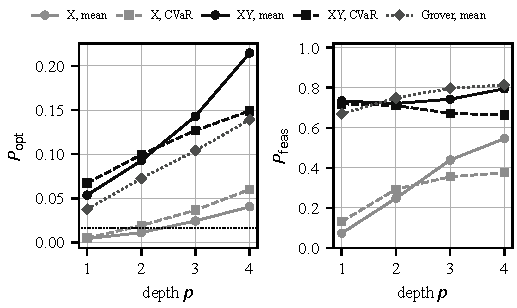
\includegraphics[width=0.92\columnwidth]{fig_popt.pdf}
\caption{Probability of the optimal plan (left, different $y$-range) and of any feasible plan (right) against depth, optimizer seed 0. Dotted: uniform one-hot.}
\label{fig:popt}
\end{figure}

The Grover mixer reached \GMMeanFour{} at $p=4$, and its difference from XY was not significant at any depth (Holm-adjusted $p\ge\StXYvGMMinP$). The data lean towards XY: at $p=4$ it was ahead on \GmWinsFour{} of \NPaired{} instances, with a mean difference of \GmDiffFour{} (paired bootstrap interval \GmDiffLo--\GmDiffHi) and an unadjusted $p=\GmRawP$. Its success@\Shots{} was higher, but a layer costs \CnotGM{} CNOTs and \NAnc{} ancillas against \CnotXY{} CNOTs.

CVaR training lowered the XY mixer's mean $P_{\mathrm{opt}}$ but raised success@\Shots{} from \QXYMeanFourSucc\% to \QXYCvarFourSucc\% (seed 0): the worst instance (capacity-binding, like all the worst) rose from \XYMin{} to \XYCvarMin.

A smaller penalty helped the X mixer only partly: lowering the weight to $\lambda=\PenBestLam$ raised its $P_{\mathrm{opt}}$ by \PenGain$\times$ to \PenBestPopt{} at a feasibility of only \PenBestFeas, still about half of the XY result. As a bound on the cost of a capacity penalty, a mixer restricted to feasible plans reached $P_{\mathrm{opt}}=\FgFour$ at $p=4$, \FgOverUni{} times uniform sampling over the same feasible plans, and beat XY on \FgWinsFour{} of \NPaired{} instances ($p=\FgPFour$).

\subsection{Angle Transfer to Held-Out Seeds}
\begin{table*}[t]
\caption{Angles at $p=4$ on the \HoN{} held-out seeds: per-instance training against one fixed angle set chosen on the development set}
\label{tab:select}
\centering
\footnotesize
\setlength{\tabcolsep}{3.3pt}
\begin{tabular}{llccccccc}
\toprule
Variant & Angles & Needs optima & Held-out $P_{\mathrm{opt}}$ & Median paired diff. & Wins of \HoN & Holm $p$ & Leave-one-out $P_{\mathrm{opt}}$ (dev.) & s@\Shots\,\%\\
\midrule
XY, mean & per instance & no & 0.163 & & & & 0.215 & 79.7\\
 & best of 5, min.\ energy & no & 0.203 & & & & 0.245 & 84.9\\
 & L-BFGS-B & no & 0.225 & & & & & 76.9\\
 & fixed, max.\ $P_{\mathrm{opt}}$ & yes & 0.306 & +0.195 & 24 & $8.5\times10^{-4}$ & 0.292 & 100.0\\
 & fixed, min.\ energy & no & 0.264 & +0.131 & 24 & $3.8\times10^{-3}$ & 0.082 & 99.9\\
 & fixed, min.\ CVaR & no & 0.234 & +0.102 & 23 & $0.039$ & 0.164 & 99.8\\
\addlinespace[1pt]
XY, CVaR & per instance & no & 0.138 & & & & 0.149 & 97.9\\
 & fixed, max.\ $P_{\mathrm{opt}}$ & yes & 0.250 & +0.070 & 29 & $6.5\times10^{-8}$ & 0.259 & 99.8\\
 & fixed, min.\ CVaR & no & 0.250 & +0.070 & 29 & $6.5\times10^{-8}$ & 0.095 & 99.8\\
\addlinespace[1pt]
X, mean & per instance & no & 0.028 & & & & 0.040 & 50.3\\
 & fixed, max.\ $P_{\mathrm{opt}}$ & yes & 0.036 & +0.010 & 20 & $0.039$ & 0.039 & 63.6\\
 & fixed, min.\ energy & no & 0.034 & +0.006 & 21 & $0.064$ & 0.034 & 65.8\\
\bottomrule
\multicolumn{9}{l}{\scriptsize Fixed sets vs.\ per-instance training of the same variant (Wilcoxon signed-rank, Holm over \SelFamily{} rows). Per-instance rows: development-set mean in the leave-one-out column.}\\
\end{tabular}
\end{table*}

Table~\ref{tab:select} gives the held-out test. For the XY mixer with the mean objective, the set chosen by (\ref{eq:transfer}) reached $P_{\mathrm{opt}}=\SelPopt$ against \SelTrained{} for per-instance training with \HoCumFour{} evaluations (better on \SelPoptWins{} of \HoN, median difference \SelPoptMed, Holm $p=\SelPoptP$). The oracle-free sets also beat per-instance training on these seeds: \SelEn{} for the energy rule ($p=\SelEnP$) and \SelCv{} for the CVaR rule ($p=\SelCvP$). Leave-one-out on the development set did not confirm this: the energy rule gave \SelEnLoo{} and the CVaR rule \SelCvLoo, both below the \SelDevTrained{} of per-instance training, while rule (\ref{eq:transfer}) gave \SelPoptLoo. The same held for CVaR angles chosen by CVaR (\SelCvarCv{} on held-out seeds, \SelCvarCvLoo{} in leave-one-out against \SelCvarDevTrained). An oracle-free choice therefore gave no reliable gain, while rule (\ref{eq:transfer}) gained in both tests. Transfer did not rescue the X mixer (\SelXPopt).

Part of the gap is a mismatch of objectives: per-instance training reached a lower mean $\langle\hat E\rangle/\Delta$ than the fixed set (\EnTrained{} against \EnFixed, lower on \EnLower{} of \HoN), but across the 30 trained sets mean energy and mean $P_{\mathrm{opt}}$ had a rank correlation of only \RhoEnPopt. Stronger optimizers stayed below: best of five COBYLA seeds \SelBestFive{} (\SelBestFiveEv{} evaluations), L-BFGS-B \SelLbfgs. COBYLA started from the fixed angles did improve on them (\StrWarm{} with \StrWarmEv{} evaluations, $p=\StrWarmP$).

A fixed set can work because performance concentrates across instances: a trained set's mean $P_{\mathrm{opt}}$ on the development set predicted its mean on the held-out seeds with rank correlation \RhoDevHeld. Only \CandBeat{} of the \CandN{} trained sets beat per-instance training there (median \CandMedian), so the choice matters. The gain came mostly from capacity-binding instances: on the \HoNBind{} binding seeds per-instance training reached \HoBindTrained{} and the fixed set \HoBindFixed, on the others \HoNonBindTrained{} and \HoNonBindFixed. We repeated training, selection and the held-out test without the scaling and with division by the standard deviation of the penalty-free energies. Without scaling the fixed angles reached only \NormNoneFixed, although per-instance training still reached \NormNoneDevTrained; with the other normalisation they reached \NormStdFixed, close to our \NormDepFixed. Transfer therefore needs a common energy scale, and the two scales we tried served about equally well. The one-time cost, \OffTrain{} training and \OffCross{} selection evaluations, equals per-instance training on about \OffBreakEven{} disruptions.

\subsection{Sampling with a Feasibility Check}
On the held-out seeds at $p=4$, the best verified plan among 8 samples came within \GapFxEight\% of the optimal cost on average for the fixed XY angles, \GapTrEight\% for per-instance training and \GapUniEight\% for uniform one-hot sampling; with 128 samples per-instance training was within \GapTrBig\%. As many plans cost close to the optimum, success@$N$ is the stricter measure.


\subsection{Transfer to Real Road Networks}
With angles fixed on the twin, pooled over the \CityN{} instances, the set chosen by (\ref{eq:transfer}) reached $P_{\mathrm{opt}}=\CityFixed$ against \CityTrained{} for per-instance training (Holm $p=\CityPHolm$) and the energy-rule set \CityEnFixed{} ($p=\CityEnPHolm$). It led in only \CityPos{} of \CityK{} cities (sign test $p=\CitySignP$), so there was no gain in $P_{\mathrm{opt}}$. Per-instance training left \CityTrainedLow{} instances with $P_{\mathrm{opt}}<0.01$, the fixed set \CityFixedLow, and success@\Shots{} rose from \CitySuccTrained\% to \CitySuccFixed\% (Holm $p=\CitySuccPHolm$) and to \CityEnSucc\% for the energy rule ($p=\CityEnSuccPHolm$), in all \CitySuccPos{} cities (sign test $p=\CitySuccSignP$).


\subsection{Larger Instances and Gate Noise}
The ring-XY circuit never leaves the $3^G$ one-hot amplitudes, so we simulated it exactly in that subspace; on \SubCheckRuns{} random 12- and 15-qubit circuits it agreed with the full statevector to $\SubCheckErr$. We took \ScN{} new twin instances for each of $G=\ScGMin,\dots,\ScGMax$ groups (\ScQubitsMin{} to \ScQubitsMax{} qubits) with the same disruption, applied the 12-qubit sets of rule (\ref{eq:transfer}) and of the energy rule unchanged, and trained every instance with the procedure above (Table~\ref{tab:size}). The set of rule (\ref{eq:transfer}) beat per-instance training at every size (Holm $p\le\ScOMaxP$ over \ScFamily{} tests). The energy-rule set won on at least \ScEWinsMin{} of \ScN{} instances at every size but was significant only at \ScESigQ{} qubits. Per-instance training (about \ScEvals{} evaluations) fell below $P_{\mathrm{opt}}=0.01$ on at least \ScBigTrainedLowMin{} of \ScN{} instances from \ScBigQ{} qubits on.

\begin{table}[t]
\caption{Fixed 12-qubit angles on \ScN{} twin instances per size $n$ (qubits), XY mixer, $p=4$; fix-O: set of rule (\ref{eq:transfer}), fix-E: energy rule; $P_{\mathrm{feas}}$ of fix-O}
\label{tab:size}
\centering
\footnotesize
\setlength{\tabcolsep}{2.2pt}
\begin{tabular}{ccccccccc}
\toprule
 & \multicolumn{5}{c}{$P_{\mathrm{opt}}$} & & \multicolumn{2}{c}{s@\Shots\,\%}\\
\cmidrule(lr){2-6}\cmidrule(lr){8-9}
$n$ & trained & fix-O & Holm $p$ & fix-E & Holm $p$ & $P_{\mathrm{feas}}$ & trained & fix-O\\
\midrule
15 & 0.1110 & 0.1924 & $4.0\times10^{-3}$ & 0.1470 & $0.083$ & 0.50 & 56.7 & 99.6\\
18 & 0.0415 & 0.0670 & $0.027$ & 0.0505 & $0.083$ & 0.36 & 31.2 & 84.4\\
21 & 0.0037 & 0.0211 & $2.0\times10^{-5}$ & 0.0139 & $1.5\times10^{-3}$ & 0.13 & 9.3 & 42.5\\
24 & 0.0016 & 0.0047 & $4.0\times10^{-3}$ & 0.0034 & $5.7\times10^{-3}$ & 0.04 & 3.9 & 12.4\\
27 & 0.0013 & 0.0026 & $0.011$ & 0.0012 & $0.083$ & 0.05 & 3.5 & 7.6\\
\bottomrule
\end{tabular}
\end{table}

In absolute terms, the fixed set's mean $P_{\mathrm{opt}}$ fell by a factor of about \ScDecay{} per added group, to \ScNineO{} at \ScQubitsMax{} qubits, still a median \ScNineOGain{} times uniform one-hot sampling; from \ScBelowUniFirstQ{} qubits on it fell below uniform sampling on up to \ScBelowUniMax{} instances. Capacity explains most of the drop. From \ScBindAllFromQ{} qubits on every instance was capacity-binding, and the fixed circuit put at most \ScFeasMaxBig{} of its probability on feasible plans, since the one-hot mixer sees capacity only through the penalty, so most samples fail the verifier.

In a trajectory noise model (\TrajRuns{} runs per circuit, \TrajInst{} development instances), each two-qubit gate fails with probability $\epsilon$ and applies a random non-identity two-qubit Pauli. As each $ZZ$ and XY gate compiles to two CNOTs, $\epsilon=0.01$ means a CNOT error near 0.5\%, close to the \SycIso--\SycSim\% two-qubit errors of a superconducting processor \cite{Arute2019}. With angles trained per instance, at $\epsilon=0.01$ and $p=4$ the XY mixer kept $P_{\mathrm{opt}}=\TrajXYOne$, \TrajRatioOne$\times$ the X mixer's \TrajXOne. A global depolarising model gave a lower \TrajGlobXYOne, as many Pauli errors barely change the output.

\subsection{Encoding Exactness and Classical Baselines}
In all \ZeroPenInfeasAll{} development instances some infeasible one-hot plan had zero penalty: three groups whose pairs fit overloaded a shelter together. Such plans usually cost more than the optimum, so the minimiser of (\ref{eq:qubo}) was the true optimum in \QuboExact\% of instances. Exhaustive search took \ExactMs~ms per instance. The greedy rule found a feasible plan in \GreedyFeas\% of instances and the optimum in \GreedyOpt\%. Bit-flip SA ended at the optimum in \SATunedOpt\% of instances and one-hot SA in \SAohOpt\%, the encoding's limit; both visited the optimum every time, so keeping the cheapest verified plan found it in \SAohVer\%.

On the \ExN{} city instances, the minimal-set penalty (\ref{eq:hubo}) was exact on every instance, checked over all 81 one-hot plans, while the pairwise penalty admitted \ExMissPlans{} infeasible penalty-free plans in \ExMissInst{} instances and its minimiser was optimal in only \ExMinPair\%. Exhaustive search took \ExExactMs~ms per instance and HiGHS \ExMilpMs~ms; both returned the optimum every time. Table~\ref{tab:exact} trains ring-XY on both penalties. The exact one raised $P_{\mathrm{feas}}$ from \ExTrFeasPair{} to \ExTrFeasHubo{} (Holm $p=\ExTrFeasP$), in all \ExFeasCities{} cities, but not $P_{\mathrm{opt}}$ (\ExTrOptPair{} against \ExTrOptHubo, $p=\ExTrOptP$), and success@\Shots{} went from \ExSuccPair\% to \ExSuccHubo\% ($p=\ExSuccP$). It helped the \ExNBind{} capacity-binding instances ($P_{\mathrm{opt}}$ \ExBindPair{} to \ExBindHubo) and hurt the others (\ExNonBindPair{} to \ExNonBindHubo). Its higher-order terms cost \ExCnotHubo{} CNOTs per layer (up to \ExCnotHuboMax) against \ExCnotPair, and a slack encoding would add \ExSlackMin{} to \ExSlackMax{} qubits to the 12.

\begin{table}[t]
\caption{Pairwise vs.\ exact capacity penalty, \ExN{} city instances, $p=4$. miss: instances with an infeasible penalty-free plan; min.: minimiser optimal}
\label{tab:exact}
\centering
\footnotesize
\setlength{\tabcolsep}{2.2pt}
\begin{tabular}{lccccccc}
\toprule
 & & & & \multicolumn{2}{c}{trained} & \multicolumn{2}{c}{fix-O}\\
\cmidrule(lr){5-6}\cmidrule(lr){7-8}
Penalty & miss & min.\,\% & CNOT & $P_{\mathrm{feas}}$ & $P_{\mathrm{opt}}$ & $P_{\mathrm{feas}}$ & $P_{\mathrm{opt}}$\\
\midrule
Pairwise & 47 & 74 & 28 & 0.601 & 0.219 & 0.571 & 0.202\\
Exact & 0 & 100 & 66 & 0.922 & 0.169 & 0.675 & 0.177\\
Holm $p$ & & & & $1.5\times10^{-6}$ & $0.081$ & $5.4\times10^{-3}$ & $0.034$\\
\bottomrule
\end{tabular}
\end{table}

\section{Discussion and Limitations}
Three findings matter for hardware experiments. First, the one-hot constraint belongs in the mixer: at the same CNOT count, ring-XY beat the transverse-field mixer on almost every instance and seed. Capacity is harder. The feasible-subspace mixer doubled $P_{\mathrm{opt}}$ but needs the feasible set; once capacity bound on every instance, ring-XY put almost all its probability on infeasible plans; and the exact penalty fixed feasibility at 12 qubits but not $P_{\mathrm{opt}}$, for more than twice the CNOTs. A capacity-aware mixer is the next step. Second, transfer needs a common energy scale and a good selection rule: with development-set optima one fixed set beat per-instance training for a one-time cost of \OffTotal{} evaluations, but without optima the gain was not reliable. Third, the pairwise penalty admits infeasible penalty-free plans, so every sample must be verified.

The exact penalty was tested on the 12-qubit city instances only. All twin instances share one disruption pattern, and the city instances use sampled demand. The noise model charges errors per logical gate, ignores single-qubit and correlated errors and was run at 12 qubits; no circuit was compiled for hardware. $P_{\mathrm{opt}}$ depends on the training budget, and the Grover test cannot prove equivalence.

\section{Conclusion}
Ring-XY gave QAOA a significantly higher $P_{\mathrm{opt}}$ than the transverse-field mixer at equal CNOT count, and angles fixed with development-set optima beat per-instance training up to \ScQubitsMax{} qubits. Capacity is the open problem: the pairwise penalty needs a verifier, and an exact penalty raised feasibility but not $P_{\mathrm{opt}}$. The results guide hardware experiments and show no present-day advantage.

\section*{Acknowledgment}
We thank the OpenStreetMap contributors and Open-Meteo for open data used by the twin.
In line with the IEEE policy on AI-generated content, the authors disclose that Claude (Anthropic) was used to help edit and restructure the text of all sections and to draft the simulation, experiment and plotting scripts. All experiments are reproducible with fixed seeds. The authors checked every number, claim and reference and take full responsibility for the content.

\balance
\begin{thebibliography}{00}
\bibitem{Lucas2014} A. Lucas, ``Ising formulations of many NP problems,'' \textit{Front. Phys.}, vol. 2, Art. no. 5, 2014, doi: 10.3389/fphy.2014.00005.
\bibitem{Glover2019} F. Glover, G. Kochenberger, and Y. Du, ``Quantum bridge analytics I: A tutorial on formulating and using QUBO models,'' \textit{4OR}, vol. 17, no. 4, pp. 335--371, 2019, doi: 10.1007/s10288-019-00424-y.
\bibitem{Cadelina2024} A. R. Cadeli\~{n}a \textit{et al.}, ``D-Wave implementation of quantum annealing for optimal resource allocation in disaster response operation of Marikina City,'' \textit{ECTI Trans. Comput. Inf. Technol.}, vol. 18, no. 1, pp. 24--33, 2024, doi: 10.37936/ecti-cit.2024181.253577.
\bibitem{Abbas2024} A. Abbas \textit{et al.}, ``Challenges and opportunities in quantum optimization,'' \textit{Nat. Rev. Phys.}, vol. 6, pp. 718--735, 2024, doi: 10.1038/s42254-024-00770-9.
\bibitem{Farhi2014} E. Farhi, J. Goldstone, and S. Gutmann, ``A quantum approximate optimization algorithm,'' arXiv:1411.4028, 2014.
\bibitem{Hadfield2019} S. Hadfield, Z. Wang, B. O'Gorman, E. G. Rieffel, D. Venturelli, and R. Biswas, ``From the quantum approximate optimization algorithm to a quantum alternating operator ansatz,'' \textit{Algorithms}, vol. 12, no. 2, Art. no. 34, 2019, doi: 10.3390/a12020034.
\bibitem{WangZ2020} Z. Wang, N. C. Rubin, J. M. Dominy, and E. G. Rieffel, ``XY mixers: Analytical and numerical results for the quantum alternating operator ansatz,'' \textit{Phys. Rev. A}, vol. 101, no. 1, Art. no. 012320, 2020, doi: 10.1103/PhysRevA.101.012320.
\bibitem{Fuchs2022} F. G. Fuchs, K. O. Lye, H. M. Nilsen, A. J. Stasik, and G. Sartor, ``Constraint preserving mixers for the quantum approximate optimization algorithm,'' \textit{Algorithms}, vol. 15, no. 6, Art. no. 202, 2022, doi: 10.3390/a15060202.
\bibitem{Bartschi2020} A. B\"{a}rtschi and S. Eidenbenz, ``Grover mixers for QAOA: Shifting complexity from mixer design to state preparation,'' in \textit{Proc. IEEE Int. Conf. Quantum Comput. Eng. (QCE)}, 2020, pp. 72--82, doi: 10.1109/QCE49297.2020.00020.
\bibitem{Sherali1991} H. D. Sherali, T. B. Carter, and A. G. Hobeika, ``A location-allocation model and algorithm for evacuation planning under hurricane/flood conditions,'' \textit{Transp. Res. B, Methodol.}, vol. 25, no. 6, pp. 439--452, 1991, doi: 10.1016/0191-2615(91)90037-J.
\bibitem{Blekos2024} K. Blekos \textit{et al.}, ``A review on quantum approximate optimization algorithm and its variants,'' \textit{Phys. Rep.}, vol. 1068, pp. 1--66, 2024, doi: 10.1016/j.physrep.2024.03.002.
\bibitem{Fuchs2024} F. G. Fuchs and R. Pariente Bassa, ``LX-mixers for QAOA: Optimal mixers restricted to subspaces and the stabilizer formalism,'' \textit{Quantum}, vol. 8, Art. no. 1535, 2024, doi: 10.22331/q-2024-11-25-1535.
\bibitem{doCarmo2025} R. S. do Carmo, M. C. S. Santana, F. F. Fanchini, V. H. C. de Albuquerque, and J. P. Papa, ``Warm-starting QAOA with XY mixers: A novel approach for quantum-enhanced vehicle routing optimization,'' arXiv:2504.19934, 2025.
\bibitem{Gupta2026} A. Gupta and S. R. Hassan, ``Constraint-preserving QAOA for personnel rostering: Coverage-preserving and guarded-XY mixer constructions,'' arXiv:2607.09145, 2026.
\bibitem{Zhou2020} L. Zhou, S.-T. Wang, S. Choi, H. Pichler, and M. D. Lukin, ``Quantum approximate optimization algorithm: Performance, mechanism, and implementation on near-term devices,'' \textit{Phys. Rev. X}, vol. 10, no. 2, Art. no. 021067, 2020, doi: 10.1103/PhysRevX.10.021067.
\bibitem{Barkoutsos2020} P. K. Barkoutsos, G. Nannicini, A. Robert, I. Tavernelli, and S. Woerner, ``Improving variational quantum optimization using CVaR,'' \textit{Quantum}, vol. 4, Art. no. 256, 2020, doi: 10.22331/q-2020-04-20-256.
\bibitem{Egger2021} D. J. Egger, J. Mare\v{c}ek, and S. Woerner, ``Warm-starting quantum optimization,'' \textit{Quantum}, vol. 5, Art. no. 479, 2021, doi: 10.22331/q-2021-06-17-479.
\bibitem{Brandao2018} F. G. S. L. Brand\~{a}o, M. Broughton, E. Farhi, S. Gutmann, and H. Neven, ``For fixed control parameters the quantum approximate optimization algorithm's objective function value concentrates for typical instances,'' arXiv:1812.04170, 2018.
\bibitem{Galda2021} A. Galda, X. Liu, D. Lykov, Y. Alexeev, and I. Safro, ``Transferability of optimal QAOA parameters between random graphs,'' in \textit{Proc. IEEE Int. Conf. Quantum Comput. Eng. (QCE)}, 2021, pp. 171--180, doi: 10.1109/QCE52317.2021.00034.
\bibitem{Shaydulin2023} R. Shaydulin, P. C. Lotshaw, J. Larson, J. Ostrowski, and T. S. Humble, ``Parameter transfer for quantum approximate optimization of weighted MaxCut,'' \textit{ACM Trans. Quantum Comput.}, vol. 4, no. 3, Art. no. 19, 2023, doi: 10.1145/3584706.
\bibitem{Harrigan2021} M. P. Harrigan \textit{et al.}, ``Quantum approximate optimization of non-planar graph problems on a planar superconducting processor,'' \textit{Nat. Phys.}, vol. 17, pp. 332--336, 2021, doi: 10.1038/s41567-020-01105-y.
\bibitem{Bartschi2019} A. B\"{a}rtschi and S. Eidenbenz, ``Deterministic preparation of Dicke states,'' in \textit{Fundamentals of Computation Theory} (LNCS, vol. 11651). Cham, Switzerland: Springer, 2019, pp. 126--139, doi: 10.1007/978-3-030-25027-0\_9.
\bibitem{Vatan2004} F. Vatan and C. Williams, ``Optimal quantum circuits for general two-qubit gates,'' \textit{Phys. Rev. A}, vol. 69, no. 3, Art. no. 032315, 2004, doi: 10.1103/PhysRevA.69.032315.
\bibitem{Nielsen2010} M. A. Nielsen and I. L. Chuang, \textit{Quantum Computation and Quantum Information}, 10th anniversary ed. Cambridge, U.K.: Cambridge Univ. Press, 2010, doi: 10.1017/CBO9780511976667.
\bibitem{Powell1994} M. J. D. Powell, ``A direct search optimization method that models the objective and constraint functions by linear interpolation,'' in \textit{Advances in Optimization and Numerical Analysis}, S. Gomez and J.-P. Hennart, Eds. Dordrecht, The Netherlands: Kluwer, 1994, pp. 51--67, doi: 10.1007/978-94-015-8330-5\_4.
\bibitem{Huangfu2018} Q. Huangfu and J. A. J. Hall, ``Parallelizing the dual revised simplex method,'' \textit{Math. Program. Comput.}, vol. 10, no. 1, pp. 119--142, 2018, doi: 10.1007/s12532-017-0130-5.
\bibitem{Kirkpatrick1983} S. Kirkpatrick, C. D. Gelatt, and M. P. Vecchi, ``Optimization by simulated annealing,'' \textit{Science}, vol. 220, no. 4598, pp. 671--680, 1983, doi: 10.1126/science.220.4598.671.
\bibitem{Arute2019} F. Arute \textit{et al.}, ``Quantum supremacy using a programmable superconducting processor,'' \textit{Nature}, vol. 574, no. 7779, pp. 505--510, 2019, doi: 10.1038/s41586-019-1666-5.
\end{thebibliography}

\end{document}
